\chapter{Proof of concept: Weakly Connected Components of a Graph}\label{prole}

One of the biggest challenges of implementing a Dynamic Pipeline is to find  a programming language with a proper set of tools supporting both of the  primary features of the \acrshort{dp}: \begin{inparaenum}[i\upshape)]
\item  \emph{parallel} processing and 
\item  \emph{strong theoretical} foundations to manage computations as first-class citizens.
 \end{inparaenum}
Haskell is a statically typed pure functional language designed on strong theoretical foundations where computations are primary entities.
This pure functional language has evolved from its birth in 1987 and nowadays provides a powerful set of tools for writing multithreading and parallel programs with optimal performance \cite{parallelbook, monadpar}. 

In the context of this research, we first assessed the suitability of \acrfull{hs}  to implement a Dynamic Pipeline. 
To be concrete, we conducted a proof of concept implementing a Dynamic Pipeline in  Haskell for solving a particular and very relevant problem as the computation/enumeration of the Weakly Connected Components of a graph.
In particular, the main objective of our proof of concept was to study the critical features required in \acrshort{hs} for a \acrshort{dpf} implementation,  the real possibilities of emitting incrementally results, and the performance of such kinds of implementations. 
Indeed, we explored the basis of an implementation of a \acrshort{dpf}  in a pure (parallel) functional language as Haskell.
This is, we determined the particular features (i.e., versions and libraries) that will allow for an efficient implementation of a \acrshort{dpf}. 
Moreover, we conducted an empirical evaluation to analyze the performance of the Dynamic Pipeline implemented in Haskell for enumerating \acrshort{wcc} with special attention to the emission of results, i.e. \acrshort{wcc}, incrementally. 
In this chapter, we focus on the presentation of our algorithm for enumerating \acrshort{wcc} using \acrshort{hs} as well as the results obtained in the empirical evaluation of its implementation. Almost all the content of this chapter is published in \cite{prole21}. 
The details of the specific requirements of the Haskell system according to the results of the proof of concept will be presented in \autoref{dp-hs}.
 
\section{$\dpwcc$ Algorithm}
Let us consider the problem of computing/enumerating the (weak) connected components of a graph $G$ using \acrshort{dp}. 
A connected component of a graph is a subgraph in which any two vertices are connected by paths. 
\begin{wrapfigure}{r}{0.4\textwidth}
  \begin{center}
\inputtikz{graph_example_wcc}
\end{center}
\caption[{[PoC] Graph WCC Example}]{Example of a graph with two weakly connected components: $\{1,2\}$ and $\{3,4,5,6\}$}
\label{fig:example_dp_graph}
\end{wrapfigure}
Thus, finding connected components of an undirected graph implies obtaining the minimal partition of the set of nodes induced by the relationship \textit{connected}, i.e., there is a path between each pair of nodes. An example of that graph can be seen in \autoref{fig:example_dp_graph}.
The input of the Dynamic Pipeline for computing the WCC of a graph, $\dpwcc$, is a sequence of edges ending with $\eof$\footnote{Note that there are neither isolated vertices nor loops in the source graph $G$.}. The connected components are output as soon as they are computed, i.e., they are produced incrementally. 
Roughly speaking the idea of the algorithm is that the weakly connected components are built in two phases. In the first phase filter instance stages receive the edges of the input graph and create sets of connected vertices. 
During the second phase, these filter instances construct maximal subsets of connected vertices, i.e. the vertices corresponding to (weakly) connected components.
%
$\dpwcc$ is defined in terms of the behavior of its four kinds stages: \textit{Source} ($\iwc$),  \textit{Generator} ($\gwc$),  \textit{Sink} ($\owc$), and \textit{Filter}($\fwc$) stages. Additionally,  the channels connecting these stages must be defined. 
In $\dpwcc$, stages are connected linearly and unidirectionally through the channels $\ice$ and  $\csofv$. Channel $\ice$ carries edges while channel  $\csofv$ conveys sets of connected vertices. Both channels end by the $\eof$ mark. 
The behavior of $\fwc$ is given by a sequence of two actors (scripts). Each actor corresponds to a phase of the algorithm. In what follows, we denote these actors by $\Act$ and $\Actt$, respectively. 
The script $\Act$ keeps a set of connected vertices ($CV$) in the state of the $\fwc$ instance. When an edge $e$ arrives, if an endpoint of $e$ is present in the state, then the other endpoint of $e$ is added to $CV$. 
Edges without incident endpoints are passed to the next stage. When $\eof$ arrives at channel $\ice$, it is passed to the next stage, and the script $\Actt$ starts its execution. 
If script $\Actt$ receives a set of connected vertices $CV$ in $\csofv$, it determines if the intersection between $CV$ and the nodes in its state is not empty. If so, it adds the nodes in $CV$  to its state. 
Otherwise, the $CV$ is passed to the next stage.  Whenever $\eof$ is received, $\Actt$ passes--through $\csofv$-- the set of vertices in its state and the $\eof$ mark to the next stage; then, it dies.
The behavior of $\iwc$ corresponds to the identity transformation over the data stream of edges.  As edges arrive, they are passed through  $\ice$ to the next stage. When receiving $\eof$ on $\ice$, this mark is put on both channels. 
Then, $\iwc$ dies. 

Let us describe this behavior with the example of the graph shown in \autoref{fig:example_dp_graph}.

\begin{figure}[h!]
  \centering
\inputtikz{dp_example_0}
\caption[{[PoC] $\dpwcc$ Initial Setup}]{$\dpwcc$ Initial setup. Stages Source, Generator, and Sink are represented by the squares labeled by $\mathsf{Sr_{WCC}}$, $\mathsf{G_{WCC}}$ and $\mathsf{Sk_{WCC}}$, respectively.  The square $\fwc$ corresponding to the Filter stage template is the parameter of $\gwc$. Arrows $\rightrightarrows$ between represents the connection of stages through two channels, $\ice$, and $\csofv$. The arrow  $\rightarrow$ represents the channel $\csofv$ connecting the stages $\mathsf{G_{WCC}}$ and $\mathsf{Sk_{WCC}}$. The arrow $\Longrightarrow$ stands for I/O data flow. Finally, the input stream comes between the dotted lines on the left and the WCC computed incrementally will be placed between the solid lines on the right.}
\label{fig:dp_example_0}
\end{figure}

\autoref{fig:dp_example_0} depicts the initial configuration of $\dpwcc$. 
The interaction of $\dpwcc$ with the "external" world is done through the stages $\iwc$ and $\owc$. 
Indeed, once activated the initial $\dpwcc$, the input stream -- consisting of a sequence containing all the edges in the graph in \autoref{fig:example_dp_graph} -- feeds $\iwc$ while  $\owc$ emits incrementally the resulting weakly connected components.  
In what follows \autoref{fig:dp_example_1_2}, \autoref{fig:dp_example_3_4}, \autoref{fig:dp_example_5_6}, \autoref{fig:dp_example_7_8} and \autoref{fig:dp_example_9_10} depict the evolution of the $\dpwcc$.
 
\begin{figure}[h!]
\centering
\begin{subfigure}[b]{\textwidth}
 \centering
  \inputtikz{dp_example_1}
  \caption{The edge $(1,2)$ is arriving to $\gwc$.}
  \label{fig:dp_example_1_2a}
\end{subfigure}
\vspace{.3cm}

\begin{subfigure}[b]{\textwidth}
 \centering
  \inputtikz{dp_example_2}
  \caption{When the edge $(1,2)$ arrives to $\gwc$, it  spawns a new instance of $\fwc$ before $\gwc$. Filter instance $F_{\{1,2\}}$ is connected to  $\gwc$ through channels $\ice$ and  $\csofv$. The state of the new filter instance $F_{\{1,2\}}$ is initialized with the set of vertices $\{1,2\}$. The edge $(3,6)$ arrives to the new filter instance $F_{\{1,2\}}$.}
  \label{fig:dp_example_1_2b}
\end{subfigure}
\caption[{[PoC] $\dpwcc$ Evolving first state}]{Evolution of the $\dpwcc$: First state}
\label{fig:dp_example_1_2}
\end{figure}
\vspace{.5cm}

\begin{figure}[h!]
\centering
\begin{subfigure}[b]{\textwidth}
 \centering
  \inputtikz{dp_example_3}
  \caption{None of the vertices in the edge $(3,6)$ is in the set of vertices $\{1,2\}$ in the state of $F_{\{1,2\}}$, hence it is passed through $\ice$ to $\gwc$.}
  \label{fig:dp_example_3_4a}
\end{subfigure}
\vspace{.3cm}

\begin{subfigure}[b]{\textwidth}
 \centering
  \inputtikz{dp_example_4}
  \caption{When the edge $(3,6)$ arrives to $\gwc$, it spawns the filter instance $F_{\{3,6\}}$  between $F_{\{1,2\}}$ and $\gwc$. Filter instance $F_{\{1,2\}}$ is connected to the new filter instance $F_{\{3,6\}}$ and this one is connected to  $\gwc$ through channels $\ice$ and  $\csofv$. The state of the new filter instance $F_{\{3,6\}}$ is initialized with the set of vertices $\{3,6\}$. The edge $(3,4)$ arrives to $F_{\{1,2\}}$  and $\mathsf{Sr_{WCC}}$ is fed with the mark $\eof$. Edges $(3,4)$ and $(4,5)$ remain passing through $\ice$.}
  \label{fig:dp_example_3_4b}
\end{subfigure}
\caption[{[PoC] $\dpwcc$ Evolving second state}]{Evolution of the $\dpwcc$: Second state}
\label{fig:dp_example_3_4}
\end{figure}
\vspace{.5cm}

\begin{figure}[h!]
\centering
\begin{subfigure}[b]{\textwidth}
 \centering
  \inputtikz{dp_example_5}
  \caption{$\mathsf{Sr_{WCC}}$  fed both, $\ice$ and $\csofv$, channels with the mark $\eof$ received from the input stream in previous state and then, it died. The edge $(4,5)$ is arriving to $\gwc$ and the edge $(3,4)$ is arriving to $F_{\{3,6\}}$. }
  \label{fig:dp_example_5_6a}
\end{subfigure}
\vspace{.3cm}

\begin{subfigure}[b]{\textwidth}
 \centering
  \inputtikz{dp_example_6}
  \caption{When the edge $(4,5)$ arrives to $\gwc$, it spawns the filter instance $F_{\{4,5\}}$  between $F_{\{3,6\}}$ and $\gwc$. Filter instance $F_{\{3,6\}}$ is connected to the new filter instance $F_{\{4,5\}}$ and this one is connected to  $\gwc$ through channels $\ice$ and  $\csofv$.  Since the edge $(3,4)$ arrived to $F_{\{3,6\}}$ at the same time and  vertex $3$ belongs to the set of connected vertices of the filter $F_{\{3,6\}}$,  the vertex $4$ is added to the state of $F_{\{3,6\}}$. Now, the state of $F_{\{3,6\}}$ is the connected set of vertices $\{3,4,6\}$. When the mark $\eof$ arrives to the first filter instance, $F_{\{1,2\}}$, through  $\csofv$, this stage passes  its partial set of connected vertices,  $\{1,2\}$, through $\csofv$ and dies.  This action will activate $\Actt$ in next  filter instances to start building  maximal connected components. In this example, the state in  $F_{\{3,6\}}$, $\{3,4,6\}$, and the arriving set $\{1,2\}$ do not intersect and, hence, both sets of vertices, $\{1,2\}$ and $\{3,4,6\}$ will be passed  to the next filter instance through $\csofv$.}
  \label{fig:dp_example_5_6b}
\end{subfigure}
\caption[{[PoC] $\dpwcc$ Evolving third state}]{Evolution of the $\dpwcc$: Third state}
\label{fig:dp_example_5_6}
\end{figure}
\vspace{.5cm}

\begin{figure}[h!]
\centering
\begin{subfigure}[b]{\textwidth}
 \centering
  \inputtikz{dp_example_7}
  \caption{The set of connected vertices  $\{3,4,6\}$ is arriving to $F_{\{4,5\}}$. The mark $\eof$ continues passing to next stages through the channel $\ice$.}
  \label{fig:dp_example_7_8a}
\end{subfigure}
\vspace{.3cm}

\begin{subfigure}[b]{\textwidth}
 \centering
  \inputtikz{dp_example_8}
  \caption{Since the intersection of the set of connected vertices $\{3,4,6\}$ arrived to  $F_{\{4,5\}}$ and its state is not empty, this state is enlarged to be $\{3,4,5,6\}$. The set of connected vertices $\{1,2\}$ is arriving to  $F_{\{4,5\}}$}
  \label{fig:dp_example_7_8b}
\end{subfigure}
\caption[{[PoC] $\dpwcc$ Evolving fourth state}]{Evolution of the $\dpwcc$:  Fourth state}
\label{fig:dp_example_7_8}
\end{figure}
\vspace{.5cm}

\begin{figure}[h!]
\centering
\begin{subfigure}[b]{\textwidth}
 \centering
  \inputtikz{dp_example_9}
  \caption{$F_{\{4,5\}}$ has passed the set of connected vertices  $\{1,2\}$ and it is arriving to $\mathsf{Sk_{WCC}}$. The mark $\eof$ is arriving to  $F_{\{4,5\}}$ through $\csofv$.}
  \label{fig:dp_example_9_10a}
\end{subfigure}
\vspace{.3cm}

\begin{subfigure}[b]{\textwidth}
 \centering
  \inputtikz{dp_example_10}
  \caption{Since the mark $\eof$ arrived to $F_{\{4,5\}}$ through $\csofv$, it passes its state, the set $\{3,4,5,6\}$ through $\csofv$ to next stages and died. The set of connected vertices  $\{1,2\}$ arrived to $\mathsf{Sk_{WCC}}$ and this implies  that $\{1,2\}$ is a maximal set of connected vertices, i.e. a connected component of the input graph. Hence,  $\mathsf{Sk_{WCC}}$ output this first weakly connected component.}
 \label{fig:dp_example_9_10b}
\end{subfigure}
\vspace{.5cm}

\begin{subfigure}[b]{\textwidth}
 \centering
  \inputtikz{dp_example_11}
  \caption{Finally, the set of connected vertices  $\{3,4,5,6\}$ arrived to $\mathsf{Sk_{WCC}}$ and was output as a new weakly connected component. Besides, the mark $\eof$ also arrived to $\mathsf{Sk_{WCC}}$ through $\csofv$ and thus, it dies.}
  \label{fig:dp_example_9_10c}
\end{subfigure}
\vspace{.3cm}

\begin{subfigure}[b]{\textwidth}
 \centering
  \inputtikz{dp_example_12}
  \caption{The weakly connected component of in the graph \autoref{fig:example_dp_graph} such as they have been emitted by $\dpwcc$.}
  \label{fig:dp_example_9_10d}
\end{subfigure}
\caption[{[PoC] $\dpwcc$ Evolving last state}]{Last states in the evolution of the $\dpwcc$}
\label{fig:dp_example_9_10}
\end{figure}

It is importat to highlight that during the states shown in \autoref{fig:dp_example_1_2a},  \autoref{fig:dp_example_1_2b},  \autoref{fig:dp_example_3_4a},  \autoref{fig:dp_example_3_4b} and  \autoref{fig:dp_example_5_6a} the only actor executed in any filter instance is $\Act$ (constructing sets of connected vertices). Afterwards, although $\Act$ can continue being executed in some filter instances, there are some instances that start executing $\Actt$ (constructing sets of maximal connected vertices). This is shown from \autoref{fig:dp_example_5_6a}  to \autoref{fig:dp_example_9_10a}.

\clearpage

\section{Empirical Evaluation}
For the empirical evaluation we consider the following research questions: 
\begin{inparaenum}[\bf {\bf RQ}1\upshape)]
\label{res:question}
    \item Does $\dpwcc$ in \acrshort{hs} support the dynamic parallelization level that $\dpwcc$ requires?
    \item Is $\dpwcc$ in \acrshort{hs} competitive compared with default implementations on base libraries for the same problem?
    \item Does $\dpwcc$ in \acrshort{hs} handle memory efficiently?
\end{inparaenum}

We have conducted different kinds of experiments to test our assumptions and verify the correctness of the implementation.
First, we have performed an \emph{Implementation Analysis} in which we have selected some graphs from \acrfull{snap} \cite{stanford} 
and analyze how the implementation behaves under real-world graphs if it timeouts or not and if it is producing correct results in terms of the amount of \acrshort{wcc} that we know beforehand.
We have also tested the implementation doing a \emph{Benchmark Analysis} where we focus on two different types of benchmarks. On the one hand, 
using \texttt{criterion} library \cite{criterion}, we have evaluated a benchmark between our solution and \acrshort{wcc} algorithm implemented in \texttt{containers} \acrshort{hs} library \cite{containers} 
using \mintinline{haskell}{Data.Graph}. On the other hand, we have compared if the results are being generated incrementally in both cases and how that is done during the pipeline execution time. 
This last analysis has been conducted using \texttt{diefpy} tool \cite{diefpaper,diefpy}.
Finally, we have executed a \textit{Performance Analysis} in which we have to gather profiling data from \acrfull{ghc} for one of the real-world graphs to measure how the program performs regarding multithreading and memory allocation.

\paragraph{Implementation analysis} The following represents the execution for running these graphs on our \acrshort{dp} implementation.

\begin{table}[H]
  \centering
  \resizebox{\textwidth}{!}{
  \begin{tabular}{|l|r|r|r|r|}
   \hline
   \textbf{Network} & \textbf{Exec Param} & \textbf{MUT Time} & \textbf{GC Time} & \textbf{Total Time}\\
   \hline
   Enron Emails & \mintinline{bash}{+RTS -N4 -s} & 2.797s & 0.942s & 3.746s \\
   \hline
   Astro Physics Coll Net & \mintinline{bash}{+RTS -N4 -s} & 2.607s & 1.392s & 4.014s \\
   \hline
   Google Web Graph & \mintinline{bash}{+RTS -N8 -s} & 137.127s & 218.913s & 356.058s \\
   \hline
  \end{tabular}
  }
 \caption[{[PoC] Execution times}]{This table shows the \acrshort{ghc} execution time measurement of selected networks. Column \texttt{Exec Param} describe the runtime flags provided to the running program. \texttt{MUT Time} is the time in seconds the program was executing computations (a.k.a. program time). \texttt{GC} Time is garbage collector time. Total time is the sum of \texttt{MUT} $+$ \texttt{GC} time.}
 \label{table:5}
 \end{table}

It is important to point out that since the first two networks are smaller in the number of edges compared with \emph{web-Google}, 
executing those with $8$ cores as the \mintinline{bash}{-N} parameters indicates does not affect the final speed-up since \acrshort{ghc} 
is not distributing threads on extra cores because it handles the load with $4$ cores only.
As we can see in \autoref{table:5}, we are obtaining remarkable execution times for the first two graphs, and it seems not to be the case 
for \textit{web-Google} due to the topology of the graph; it is denser in terms of connected components than the others.

\paragraph{Benchmark Analysis} Regarding mean execution times for each implementation on each case measure by \texttt{criterion} library \cite{criterion}, we can display the following results:

\begin{table}[H]
  \centering
  \resizebox{\textwidth}{!}{
  \begin{tabular}{|l|l|l|l|}
   \hline
   \textbf{Network} & \textbf{\acrshort{dpwcc}} & \textbf{\acrshort{hs} \texttt{containers}} & \textbf{Speed-up}\\
   \hline
   Enron Emails & 4.68s &  6.46s & 1.38\\
   \hline
   Astro Physics Coll Net & 4.98s & 6.95s  & 1.39\\
   \hline
   Google Web Graph & 386s & 106s & 0.27\\
   \hline
  \end{tabular}
  }
 \caption[{[PoC] Mean Execution times}]{Mean execution time of each network running under \texttt{criterion} library comparing both implementations in \acrshort{hs}: \acrshort{dpwcc} and \texttt{containers} lib. \texttt{criterion} runs $1000$ times each implementations and takes mean execution times of each. \texttt{Speed-up} column shows the ratio between \texttt{Haskell containers} and \texttt{\acrshort{dpwcc}}}
 \label{table:6}
 \end{table}

These results allow for answering Question [Q2], where we have seen that the graph topology is affecting the performance and the parallelization, penalizing \acrshort{dpwcc} for this particular case. In this benchmark, 
the solution against a non-parallel \texttt{containers} \mintinline{haskell}{Data.Graph} confirms the hypothesis. 

\paragraph{Diefficency metrics} Some considerations are needed before starting to analyze the data gathered with \acrfull{dt} tool. Firstly, the tool is plotting the results according to the traces generated by the implementation, 
both \acrshort{dpwcc} and \acrshort{hs} \emph{containers}. By the nature of \acrshort{dp} model, we can gather or register that timestamps as long as the model is generating results. In the case of \acrshort{hs} \texttt{containers}, this is not possible since it 
calculates \acrshort{wcc} at once. This is not an issue and we still can check at what point in time all \acrshort{wcc} in \acrshort{hs} \texttt{containers} are generated. In those cases, we are going to see a straight vertical line. 

It is important to remark that we needed to scale the timestamps because we have taken the time in nanoseconds. After all, the incremental generation between one \acrshort{wcc} and the other is very small but significant enough to be taken into consideration. 
Thus, if we left the time scale in integer milliseconds, microseconds, or nanoseconds integer part, it cannot be appreciated. In case of escalation, we are discounting the nanosecond integer of the first generated results resulting in a time scale that starts close to $0$. 
This does not mean that the first result is generated at $0$ time, but we are discarding the previous time to focus on how the results are incrementally generated.

Having said that, we can see the results of \acrshort{dt} which are presented in two types of plots. The first one is regular line graphs in where the $x$ axis shows the time that escalated when the result was generated, and the $y$ axis shows the component number that was generated at that time. 
The second type of plot is a radar plot in which shows how the solution is behaving 
on the dimensions of  \acrfull{tfft}, \acrfull{et}, \acrfull{tt}, \acrfull{comp} and \acrfull{dt} and how are the tension between them; all these metrics are higher is better. 
All the details about these metrics are explained here \cite{diefpaper}.

\begin{figure}[!htb]
    \centering
    \begin{subfigure}{0.33\textwidth}
     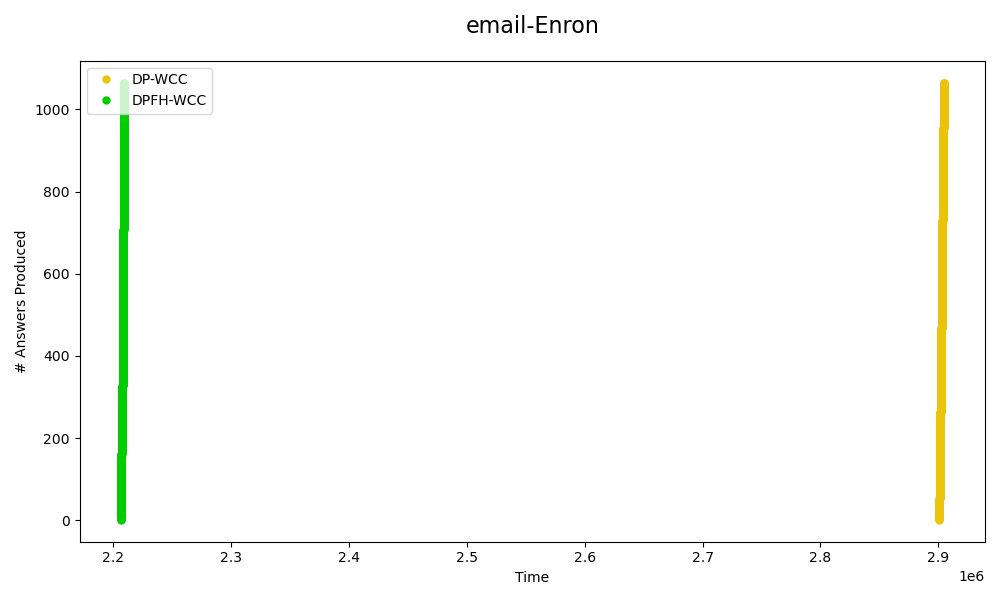
\includegraphics[width=1\linewidth, height=0.2\textheight]{email_enron}
      \caption[{[PoC] \acrshort{dt} Results: email-Enron}]{email-Enron \acrshort{dt}}
      \label{fig:dief:1}
    \end{subfigure}%
    \begin{subfigure}{0.33\textwidth}
     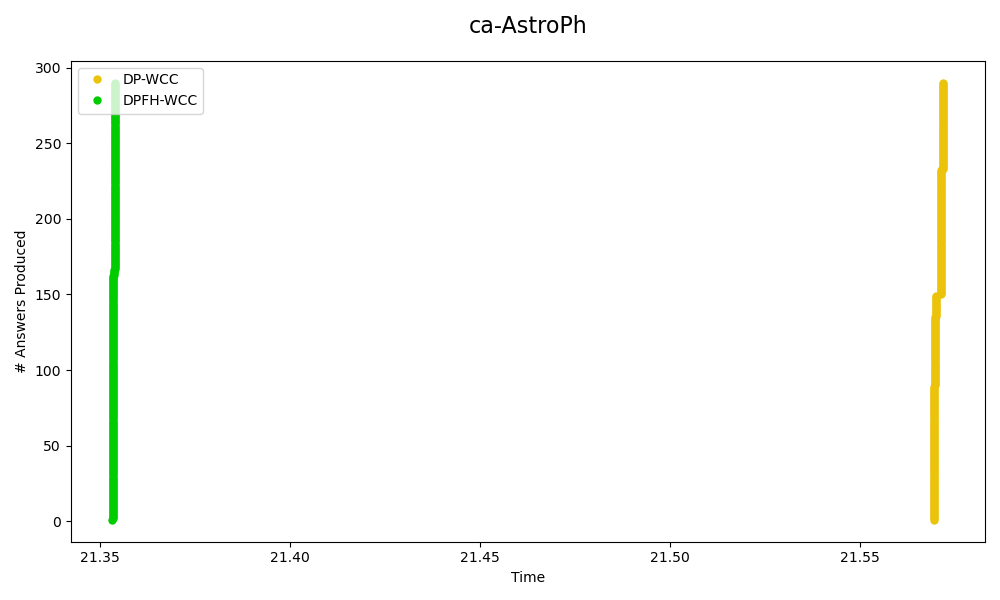
\includegraphics[width=1\linewidth, height=0.2\textheight]{ca_astroph}
      \caption[{[PoC] \acrshort{dt} Results: ca-AstroPh}]{ca-AstroPh \acrshort{dt}}
      \label{fig:dief:2}
    \end{subfigure}%
    \begin{subfigure}{0.33\textwidth}
     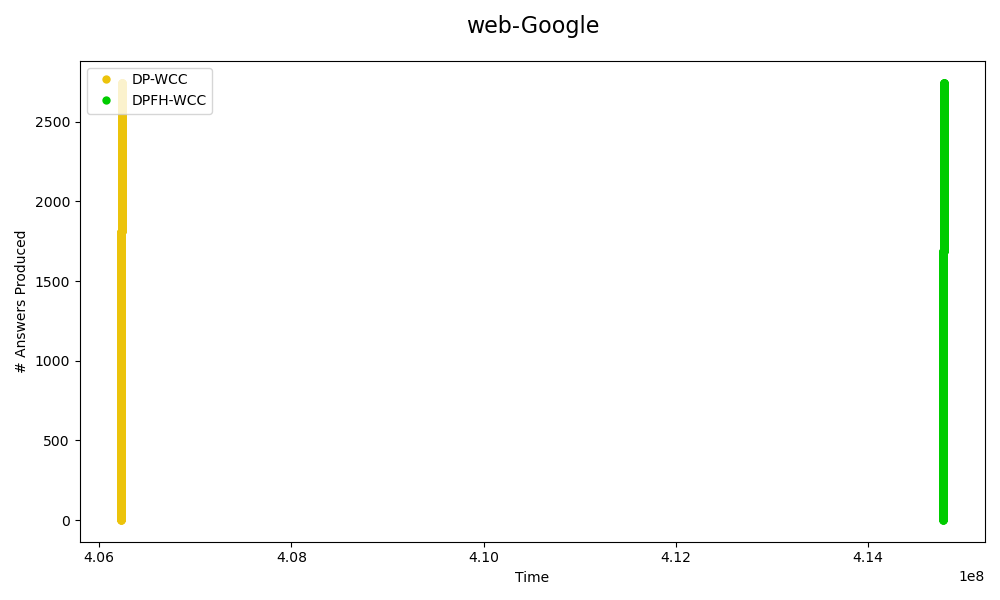
\includegraphics[width=1\linewidth, height=0.2\textheight]{web_google}
      \caption[{[PoC] \acrshort{dt} Results: web-Google}]{web-Google \acrshort{dt}}
      \label{fig:dief:3}
    \end{subfigure}
    \caption[{[PoC] \acrshort{dt} Metrics}]{This plots are showing the \acrshort{dt} on the three networks comparing both \acrshort{hs} implementations \acrshort{dpwcc} and \texttt{containers} lib. Red lines indicates \texttt{containers} \acrshort{hs} \acrshort{dt} metric. Yellow points indicates \acrshort{dpwcc} \acrshort{dt} metric}
\end{figure}

\begin{figure}[!htb]
  \centering
  \begin{subfigure}{0.33\textwidth}
   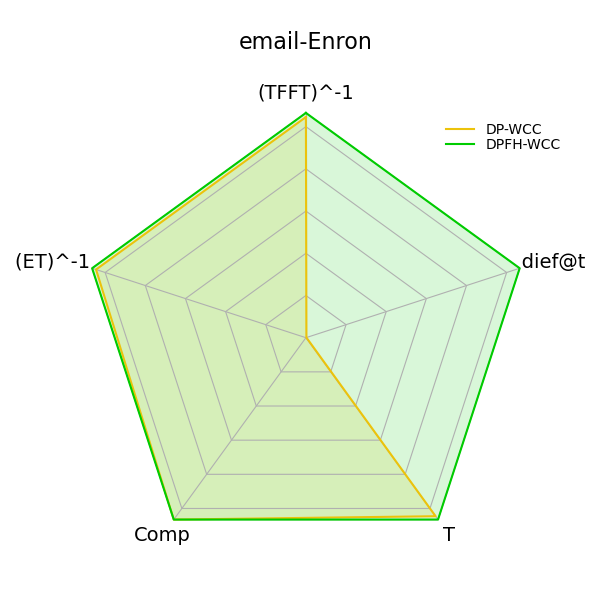
\includegraphics[width=1\linewidth, height=0.2\textheight]{email_enron_radar}
    \caption[{[PoC] \acrshort{dt} Results: email-Enron radar}]{email-Enron \acrshort{dt}}
    \label{fig:dief:rad:1}
  \end{subfigure}%
  \begin{subfigure}{0.33\textwidth}
   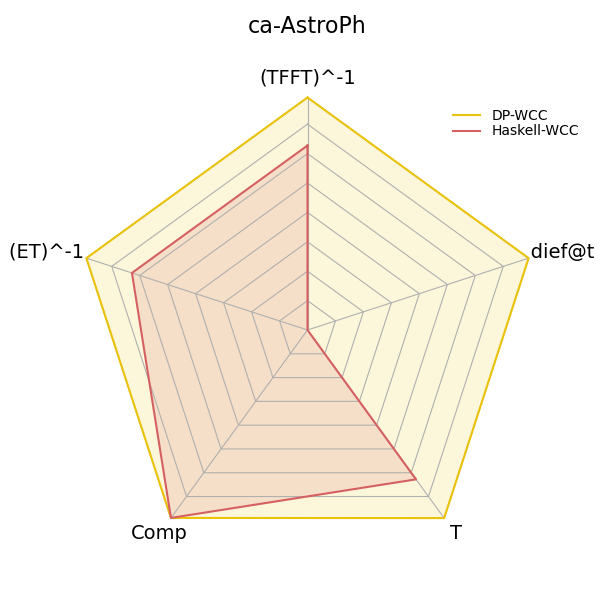
\includegraphics[width=1\linewidth, height=0.2\textheight]{ca_astroph_radar}
    \caption[{[PoC] \acrshort{dt} Results: ca-AstroPh radar}]{ca-AstroPh \acrshort{dt}}
    \label{fig:dief:rad:2}
  \end{subfigure}%
  \begin{subfigure}{0.33\textwidth}
   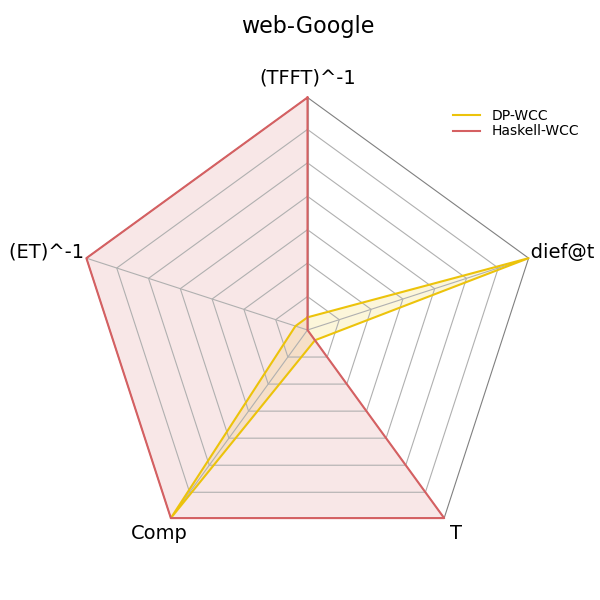
\includegraphics[width=1\linewidth, height=0.2\textheight]{web_google_radar}
    \caption[{[PoC] \acrshort{dt} Results: web-Google radar}]{web-Google \acrshort{dt}}
    \label{fig:dief:rad:3}
  \end{subfigure}
  \caption[{[PoC] \acrshort{dt} Metrics (Radial)}]{Radial plot shows how the different metrics provided by \acrshort{dt} tool such as \acrfull{tt}, \acrfull{tfft}, \acrfull{dt}, \acrfull{et} and \acrfull{comp} are related each other for each \acrshort{hs} implementation: \acrshort{dpwcc} and \texttt{containers}. Red area indicates \texttt{containers} \acrshort{hs} \acrshort{dt} metric. Yellow area indicates \acrshort{dpwcc} \acrshort{dt} metric}
\end{figure}

Based on the results shown in all the figures above, all the solutions in \acrshort{dpwcc} are being generated incrementally, 
but there is some difference that we would like to remark. In the case of \emph{email-Enron} and \emph{ca-AstroPh} graphs 
as we can see in \autoref{fig:dief:1} and \autoref{fig:dief:2}, there seems to be a more incremental generation of results. 
This behavior is measured with the values of \acrfull{dt}. \emph{ca-AstroPh} as it can be seen in \autoref{fig:dief:2}, is even more incremental, and it is showing a clear separation between some results and others. 
The \emph{web-Google} network, which is shown in \autoref{fig:dief:3}, is a little more linear, and that is because all the results are being generated with very little difference in time between them. 
Having the biggest \acrshort{wcc} at the end of \emph{web-Google} \acrshort{dp} algorithm 
it is retaining results until the biggest \acrshort{wcc} can be solved, which takes longer. 


\paragraph{Multithreading} For analyzing parallelization and multithreading we have used \textit{ThreadScope} \cite{threadscope} which allows us to see how the parallelization is taking place on \acrshort{ghc} at a fine grained level and how the threads are distributed throughout the different cores requested with the \mintinline{bash}{-N} execution \texttt{ghc-option} flag.
The distribution of the load is more intensive at the end of the execution, where \mintinline{haskell}{actor2} filter stage of the algorithm is taking place and different filters are reaching execution of that second actor.
We can appreciate how many threads are being spawned and by the tool and if they are evenly distributed among cores. 

\begin{figure}[!htb]
  \centering
  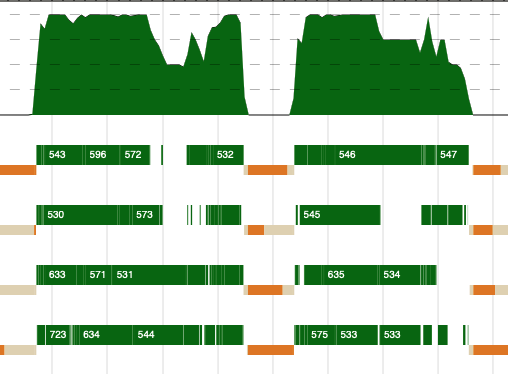
\includegraphics[width=0.7\textwidth, height=0.3\textheight]{screen_2}
  \caption[{[PoC] Thread Metrics: Fraction of Time}]{Threadscope Image of Zoomed Fraction of $10$ nanoseconds. Upper green area shows the amount of core used during that fraction of time. The lower are where it shows four separated green bars describe the behavior on each core. The number inside the green bar show the amount of threads running on that core at that moment. Finally orange bars are GC time.}
  \label{fig:4}
 \end{figure}

~\autoref{fig:4} zooms in on \textit{ThreadScope} output in a particular moment, approximately in the middle of the execution. 
The numbers inside green bars represent the number of threads that are being executed on that particular core (horizontal line) at that execution slot. 
Thus, the number of threads varies among slot execution times, because as it is already known, \acrshort{ghc} implements \emph{Preemptive Scheduling} \cite{lightweightghc}.
It can be appreciated in \autoref{fig:4} our first assumption that the load is evenly distributed because the mean number of executing threads per core is $571$.


\paragraph{Memory allocation} Another important aspect in our case is how the memory is being managed to avoid memory leaks or other non-desired behavior that increases memory allocation during the execution time. 
This is even more important in the particular implementation of \acrshort{wcc} using \acrshort{dp} model because it requires to maintain the set of connected components in memory throughout the execution of the program or at least until we can output the calculated \acrshort{wcc} if we reach to the last \textit{Filter} and we know that this \acrshort{wcc} cannot be enlarged anymore.
In order to verify this, we measure memory allocation with \textit{eventlog2html} \cite{eventlog2html} which converts generated profiling memory eventlog files into graphical HTML representation. 

\begin{figure}[!htb]
  \centering
  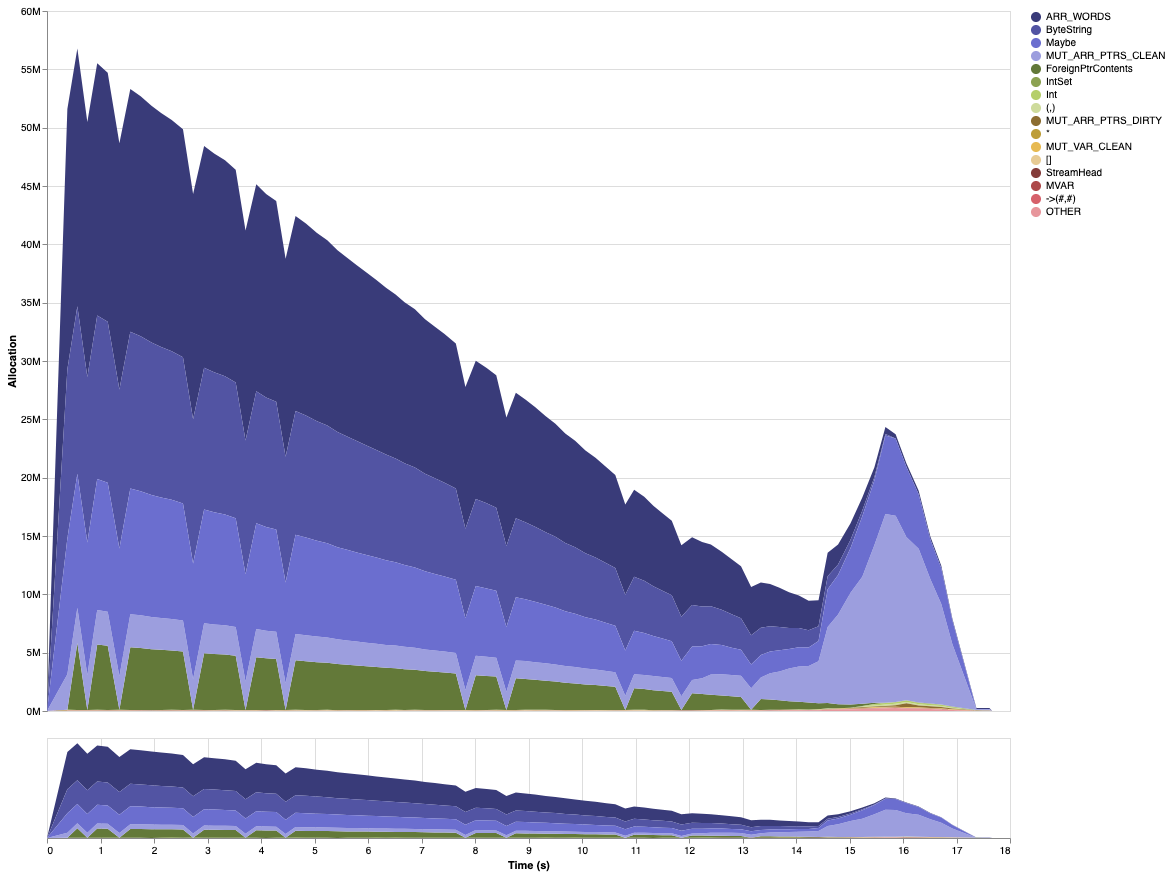
\includegraphics[width=1\linewidth, height=0.3\textheight]{visualization}
  \caption[{[PoC] Memory Metrics: Allocation by Data Type}]{This plot is showing the accumulated memory allocation size of each \acrshort{hs} Data Type throughout the execution of the program. The dark blue area shows the \texttt{ARR\_WORDS} data type which is \texttt{String} values. There are many of them because all that it comes from a file is in \texttt{String} format and need to be converted to the proper Data type. Rest of the light blue areas belong to \texttt{ByteString} which is the format treated in the input file as well, and \texttt{Maybe} type which is the type of data transfer between channels.}
  \label{fig:5}
\end{figure}

As we can see in \autoref{fig:5}, \acrshort{dpwcc} does efficient work on allocating memory since we are not using more than $57$ MB of memory during the whole execution of the program.
On the other hand, if we analyze how the memory is allocated during the execution of the program, it can also be appreciated that most of the memory is allocated at the beginning of the program and steadily decrease over time, with a small peak at the end that does not overpass even half of the initial peak of $57$ MB. 
The explanation for this behavior is quite straightforward because, in the beginning, we are reading from the file and transforming a \mintinline{haskell}{ByteString} buffer to \mintinline{haskell}{(Int, Int)} edges. 
This is seen in the image in which the dark blue that is on top of the area is \mintinline{haskell}{ByteString} allocation. 
Light blue is allocation of \mintinline{haskell}{Maybe a} type which is the type that is returned by the \textit{Channels} because it can contain a value or not. 
Data value \mintinline{haskell}{Nothing} is indicating end of the \textit{Channel}. 
Another important aspect is the green area which represents \mintinline{haskell}{IntSet} allocation, which in the case of our program is the data structure that we use to gather the set of vertices that represents a \acrshort{wcc}. 
This means that the amount of memory used for gathering the \acrshort{wcc} itself is minimum, and it is decreasing over time, which is another empirical indication that we are incrementally releasing results to the user. 
It can be seen as well that as long the green area reduces the lighter blue (\texttt{MUT\_ARR\_PTRS\_CLEAN} \cite{ghcheap}) increases at the same time indicating that the computations for the output (releasing results) is taking place. 
Finally, according to what we have stated above, we can answer the question [Q3], showing that not only the memory management was efficient, but at the same time, the memory was not leaking or increasing across the running execution program.

The empirical evaluation of the \acrshort{dpwcc} implementation to compute weakly connected components of a graph, evidence suitability, 
and robustness to provide a Dynamic Pipeline Framework in that language. Measuring using \par\bigskip metrics reveals some advantageous capability of $\dpwcc$ implementation to deliver incremental results compared with default containers library implementation. 
Regarding the main aspects where DPP is strong, i.e., pipeline parallelism and time processing, the $\dpwcc$ performance shows that Haskell 
can deal with the requirements for the \acrshort{wcc} problem without penalizing neither execution time nor memory allocation. 
In particular, the $\dpwcc$ implementation outperforms in those cases where the topology of the graph is sparse and where the number of vertices in the largest \acrshort{wcc} is not big enough. 
To conclude, the proof of concept has gathered enough evidence to show that the implementation of Dynamic Pipeline in Haskell Programming Language is feasible. 
This fact opens a wide range of algorithms to be explored using the Dynamic Pipeline Paradigm, supported by purely functional programming language.

\section{Chapter Summary}
In this chapter, we have presented a proof of concept that allows us to assess the feasibility of implementing \acrshort{dp} using \acrshort{hs}. 
The obtained results gave us insights about how to proceed for implementing a first version of a DPF using (parallel) Haskell and, afterward, to implement an algorithm for enumerating incrementally the bitriangles of a bipartite graph based on the  \acrshort{dp}.

